%!TEX TS-program = xelatex
%!TEX encoding = UTF-8 Unicode

\documentclass[11pt]{extarticle}
% extarticle is like article but can handle 8pt, 9pt, 10pt, 11pt, 12pt, 14pt, 17pt, and 20pt text

\def \ititle {Mindreading \& Joint Action: Philosophical Tools}
\def \isubtitle {Lecture 7: What Is Shared Agency?}
\def \iauthor {Stephen A. Butterfill}
\def \iemail{s.butterfill@warwick.ac.uk}
\date{}

\input{$HOME/Documents/submissions/preamble_steve_handout}

%for strikethrough
\usepackage[normalem]{ulem}

%itemize bullet should be dash
\renewcommand{\labelitemi}{$-$}

\begin{document}

\begin{multicols}{3}

\setlength\footnotesep{1em}

\bibpunct{}{}{,}{s}{}{,}  %use superscript TICS style bib

\bibliographystyle{newapa} %apalike

%\maketitle
%\tableofcontents






\begin{center}
{\Large
Mindreading \& Joint Action: Philosophical Tools}

Lecture 9: Interacting Mindreaders


ButterfillS@ceu.hu
\end{center}


\section{Aim}
Show that capacities for pure goal ascription and shared agency could explain the emergence of minimal theory of mind, and of simple forms of communication.



\begin{center}
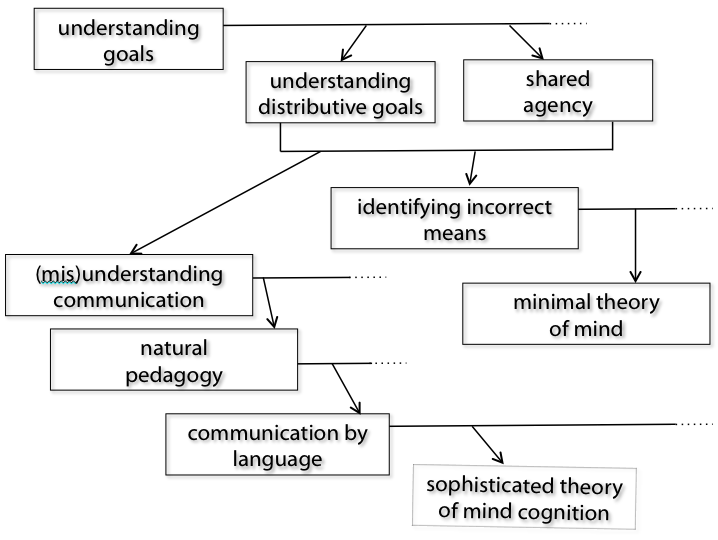
\includegraphics[width=8cm]{fig_emergence.png}

\end{center}



\section{Recap: shared agency}
There is a form of shared agency exercises of which do involve no shared intention, nor any mindreading beyond pure goal ascription (see Lecture 8).



\section{Recap: goal ascription}

\newcommand{\dfGoalAscription}{\emph{Goal ascription} is the process of identifying outcomes to which purposive actions are directed as outcomes to which those actions are directed.}

\dfGoalAscription{}

\emph{Pure} goal ascription is goal ascription which occurs independently of any knowledge of mental states.

Let $R{_M}(a,G,s)$ be the relation that holds just if: (i) were $M$  tasked with producing $G$ in situation $s$, then it would plan action $a$; and (ii) $G$ is desirable.

Claim: pure goal ascription depends on using one's own planning mechanisms to compute this family of relations $R{_M}$.


\section{Limits of Pure Goal Ascription}



\subsection{The Problem of False Belief}
Differences between what an observer and an actor believe can be an obstacle to goal ascription.


\subsection{The Problem of Opaque Means}
Ignorance about to which ends actions are means can be an obstacle to goal ascription. 
This problem affects (i) tool use and (ii) communication.


\section{Your-goal-is-my-goal}
\begin{enumerate}
\item You are willing to engage in some joint action* or other with me.
%(for example, because you have made eye contact with me while I was in the middle of attempting to do something).

\item I am not about to change the single goal to which my actions will be directed.

\end{enumerate}
%
Therefore:
%
\begin{enumerate}[resume]
%
\item A goal of your actions will be my goal, the goal I now envisage that my actions will be directed to.
\end{enumerate}
%

[*Any conception of joint action on which joint actions involve distributive goals will do.]


\section{Application: communication}

`to understand pointing, the subject needs to understand more than the individual goal-directed behaviour. She needs to understand that ... the other attempts to communicate to her ...  and ... the communicative intention behind the gesture'\citep{Moll:2007gu}


\begin{center}
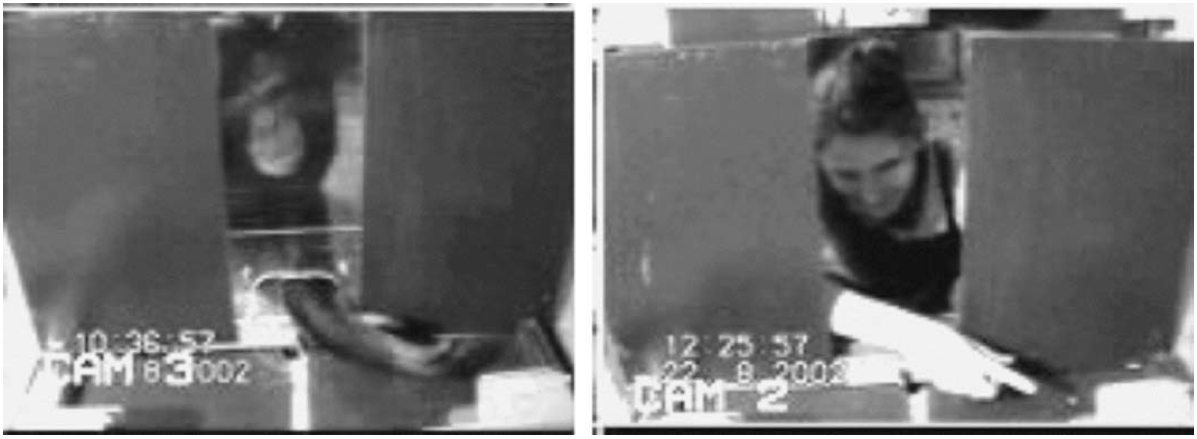
\includegraphics[width=6cm]{figure_hare_toma_2004_e3.png}
\label{fig:reach_point}

A failed reach (left) and a helpful point (right).\citep%[p.\ 557, figure 4]
	{hare_chimpanzees_2004}
\end{center}



Leekam et al.: `the adult’s social cues conveyed her communicative intent, which in turn encouraged the child to `see through the sign'.'
\citep%[p.\ 118]
{leekam_adults_2010}


\section{Natural Pedagogy: Ingredients}
\textbf{ostension} `the teacher has to explicitly mark her behaviour as being a pedagogical manifestation ...\  communication makes manifest not just the intended message content but also the communicative intent of the speaker’ \citep{Csibra:2005zr} %[p.\ 6]

\textbf{reference} `the teacher ...\ has to specify what she is teaching about.’ \citep{Csibra:2005zr} %[p.\ 6]

\textbf{relevance}:  ‘Manifesting knowledge content and disambiguating such manifestation can rely on the mutually shared understanding between teacher and learner that ...\ the teacher's communication conveys novel and relevant knowledge to the learner.’ \citep{Csibra:2005zr} %[p.\ 7]


\section{Natural Pedagogy \& Reference}
What is the relation between a communicative action and its referent?
(Compare: We might characterise the relation between an action and its goal by appeal to intention, motor representation or teleological function, and we can explain how this relation can be tracked using the Principle of Rationality.)



\section{Natural Pedagogy \& Opaque Means}
Natural pedagogy shows that if we can solve the problem of opaque means for communication, we can solve it for tool use too.
But this hypothesis doesn't explain how the problem of opaque means is solved for communication.



\section{Natural Pedagogy \& Mindreading}
Natural pedagogy does \emph{not} require mindreading:
‘the ability to teach and to learn from teaching is a primary, independent, and possibly phylogenetically even earlier adaptation than ...\ the ability to attribute mental states.'\citep{Gergely:2012np} %(Gergely & Csibra 2012: 2)

Natural pedagogy \emph{does} require mindreading:
`the assumption of relevance requires the learner to decode the teacher's manifestation with respect to his own knowledge.  ...  the pedagogical question driving the learner's inferential interpretation of the teacher’s demonstration is this: ``What is the new information in this manifestation that I don’t yet know and would not be able to figure out myself?'''\citep{Csibra:2005zr} %(Csibra & Gergely 2005: 7)

Natural pedagogy \emph{does} require mindreading:
`infants, by decoding ostensive signals, recognize the communicative intentions of communicators ... Attributing a communicative intention is attributing a second-order intention'\citep{csibra:2010_recognizing} %(Csibra 2010: 160)

%`When perceiving an ostensive cue, infants minimally have to be able to interpret it as indicating a second order intention referring to the presence of further signals that carry some communicative ... content (Csibra, 2010).' (Gergely \& Csibra 2012: 7)





\footnotesize 
\bibliography{$HOME/endnote/phd_biblio}

\end{multicols}

\end{document}